\documentclass{beamer}

\usepackage[utf8]{inputenc}
\usetheme{Warsaw}
\graphicspath{{/home/marvin/neuro-seg/Soutenance/}}
\setbeamersize{text margin left=1.4cm}
\begin{document}
\setbeamertemplate{navigation symbols}{}
\setbeamertemplate{footline}[frame number]

\title[Signal segmentation]{Functional data analysis applied to neurology}
\author{Clément Bonvoisin, Pierre Ludmann}
\institute{CMLA (ENS Cachan), Cognac-G (Paris V)}
\date{30 juin 2014}

\begin{frame}
\titlepage
\end{frame}

\begin{frame}
\frametitle{Plan}
  \tableofcontents[hideallsubsections]
\end{frame}

\AtBeginSection[]
{
  \begin{frame}
  \tableofcontents[currentsection, hideothersubsections]
  \end{frame} 
}


\section{Introduction}

	\subsection{Introduction au problème}

\begin{frame}
	\frametitle{Présentation du problème}
	\begin{itemize}
		\item[Projet] pluridisciplinaire
			\\ Médecins
			\\ Mathématiciens
		\item[Enjeux] variés
			\\ Fournir une base de donnée aux deux acteurs
			\\ Tester des modèles sur des signaux réels
			\\ Suivi des patients
			\\ Étudier les troubles de la marche
		\item[Protocole] expérimental
			\\ Placements des capteurs
			\\ Mouvements
			\\ Référentiel de travail
	\end{itemize}	
\end{frame}

	\subsection{Segmentation d'un signal}

\begin{frame}
	\frametitle{Exemple sur des signaux physiologiques}
	\begin{figure}
		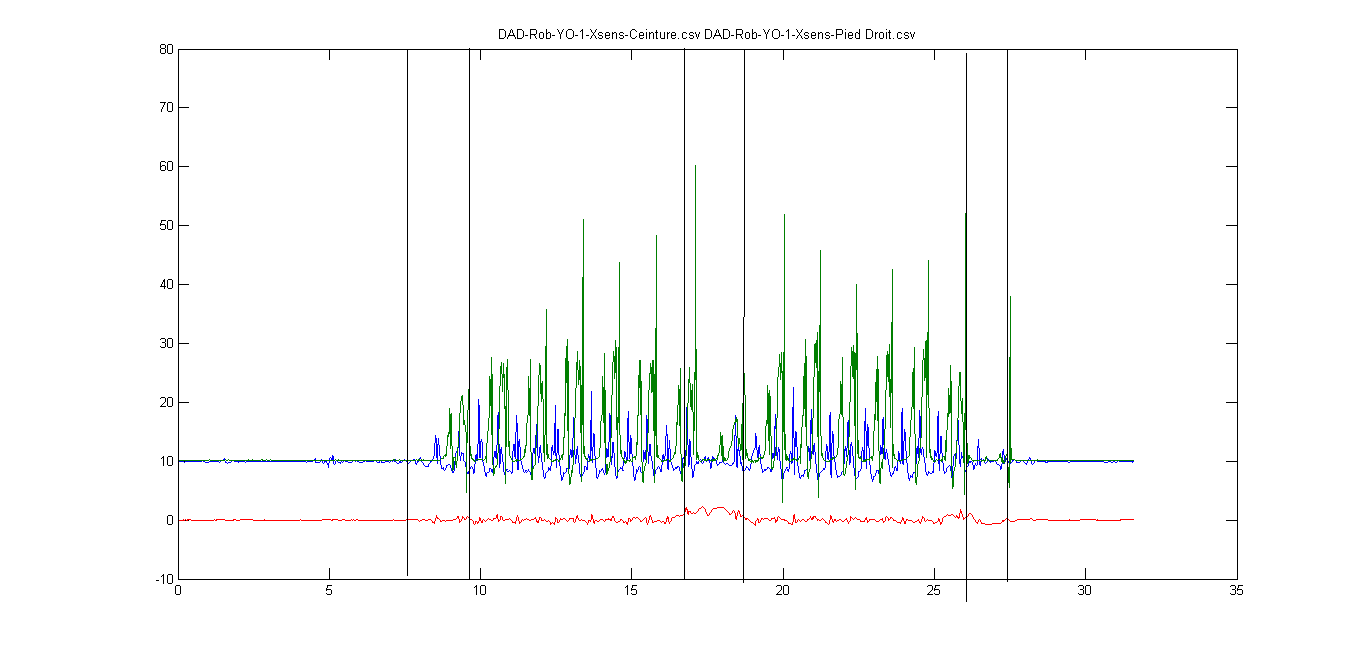
\includegraphics[scale=0.3]{exemple_seg.png}
		\caption{Segmentation à la main d'un signal de marche}
	\end{figure}
\end{frame}


%\begin{frame}
%	\frametitle{}
%	\begin{itemize}
%		\item[L'affichage] montre clairement les différentes séquences de l'expérience
%		\item[$\Longrightarrow$] La segmentation automatique doit être rapide et précise, au moins autant qu'à l'œil
		
%		\item[Etiquettes]: Idle, Start, Stop, Walk, Turn, Trash
	
%	\end{itemize}
%\end{frame}

\section{Formalisation et outils}

\subsection{Définition}

\begin{frame}

\frametitle{Formaliser les ruptures}

\begin{itemize}
	\item[Signaux] réalisations d'un nombre fini de variables aléatoires
\end{itemize}

\vspace{-.4cm}
\[ (X_n)_{n \in [\![ 1\,; N ]\!] } \]
\phantom{kcahkcah}
	
\begin{itemize}
	\item[Ruptures]aux $R$ instants $t_r$ où la loi des variables aléatoires $X_i$ change.
\end{itemize}

\vspace{-.4cm}
\[ \forall r \in [\![0\,;R-1]\!] , (X_n)_{n\in[\![t_{r-1}\,;t_r]\!]} \sim p_r\]
\hspace{.7cm}
où $t_{-1}=1$ et $t_R=N$

%\[	\forall n \in [\![1\,; t_0-1]\!], X_n \sim p_0 \]
%\[	\forall n \in [\![t_0\,; N]\!], X_n \sim p_1 \]

\end{frame}

\subsection{Algorithme CUSUM}

\begin{frame}

	\frametitle{Une détection par CUSUM hors-ligne}

	\begin{itemize}
%		\item[Biblio] \emph{Detection of Abrupt Changes : Theory and Application},\\
%		M. Basseville, I. V. Nikiforov (1993)
%		\item[Proposé] dans \emph{Continuous inspection scheme}, E.S. Page (1954)
		\item[Comparer] l'hypothèse d'une rupture à l'hypothèse de non-rupture
	\end{itemize}

\vspace{-.4cm}
	\begin{equation}
		L _k =\ln \left[ \frac{\sup_{\theta_0}\left\{ \prod_{i=1}^{k-1} p_{\theta_0}(y_i) \right\} \cdot \sup_{\theta_1} \left\{ \prod_{i = k}^{N}p_{\theta_1}(y_i) \right\}}{\sup_{\tilde\theta}\left\{\prod_{i=i}^{N}p_{\tilde{\theta}}(y_i)\right\}} \right]
	\end{equation}
\phantom{kcahkcah}

	\begin{itemize}
		\item[Rupture] au temps de vraisemblance logarithmique maximale
	\end{itemize}

\vspace{-.4cm}
	\begin{equation}
		t_0 = \arg \max_{1 \leq k \leq N} L_k
	\end{equation}
	
\end{frame}

\subsection{Hypothèses et conséquences}

\begin{frame}
	\frametitle{Hypothèses de travail}
	
	\begin{itemize}
		\item[Hypothèse] forte d'indépendance temporelle et spatiale
		\item[Hypothèse] de signaux supposés suivre une distribution normale :
	\begin{equation}
		p_{\mu, \sigma}(y) = \frac1{\sigma\sqrt{2 \pi}} \exp \left[ -\frac12 \left( \frac{y - \mu}{\sigma} \right)^2 \right]
	\end{equation}
		\item[$\Longrightarrow$] bornes supérieures atteintes aux estimateurs
		\vspace{.4cm}
		\item[Paramètre] $\theta$ : changement de la moyenne et/ou de l'écart-type du signal
	\end{itemize}
\end{frame}

\begin{frame}
	\frametitle{Choix des paramètres - Formules correspondantes}
	Trois choix possibles :
	\vspace*{.3cm}
	\begin{itemize}
		\item[$\theta=\mu$]: (4) avec $\mu=\frac1n\sum_{i=1}^ny_i$ et $\sigma$ fixé
		\vspace*{.2cm}
		\item[$\theta=\sigma$]:  (5) avec $\mu$ fixé et $\sigma=\frac1n\sum_{i=1}^n(y_i-\mu)^2$
		\vspace*{.2cm}
		\item[$\theta=(\mu,\theta)$]: (5) avec \mbox{$\mu=\frac1n\sum_{i=1}^ny_i$ et $\sigma=\frac1n\left[\sum_{i=1}^ny_i^2-(\sum_{i=1}^ny_i)^2\right]$}
	\end{itemize}
	\vspace*{0.8cm}
	\begin{equation}
	\hspace{-1cm}	L_k=\frac 1{2\sigma^2}\left[(k-1)\mu_0^2+(N-k+1)\mu_1^2-N\tilde\mu^2\right]
	\end{equation}
	ou
	\begin{equation}
	\hspace{-1cm}	L_k=N\ln(\tilde\sigma)-(k-1)\ln(\sigma_0)-(N-k+1)\ln(\sigma_1)
	\end{equation}
\end{frame}

\begin{frame}
	\frametitle{Détection d'une rupture}
	\begin{figure}
		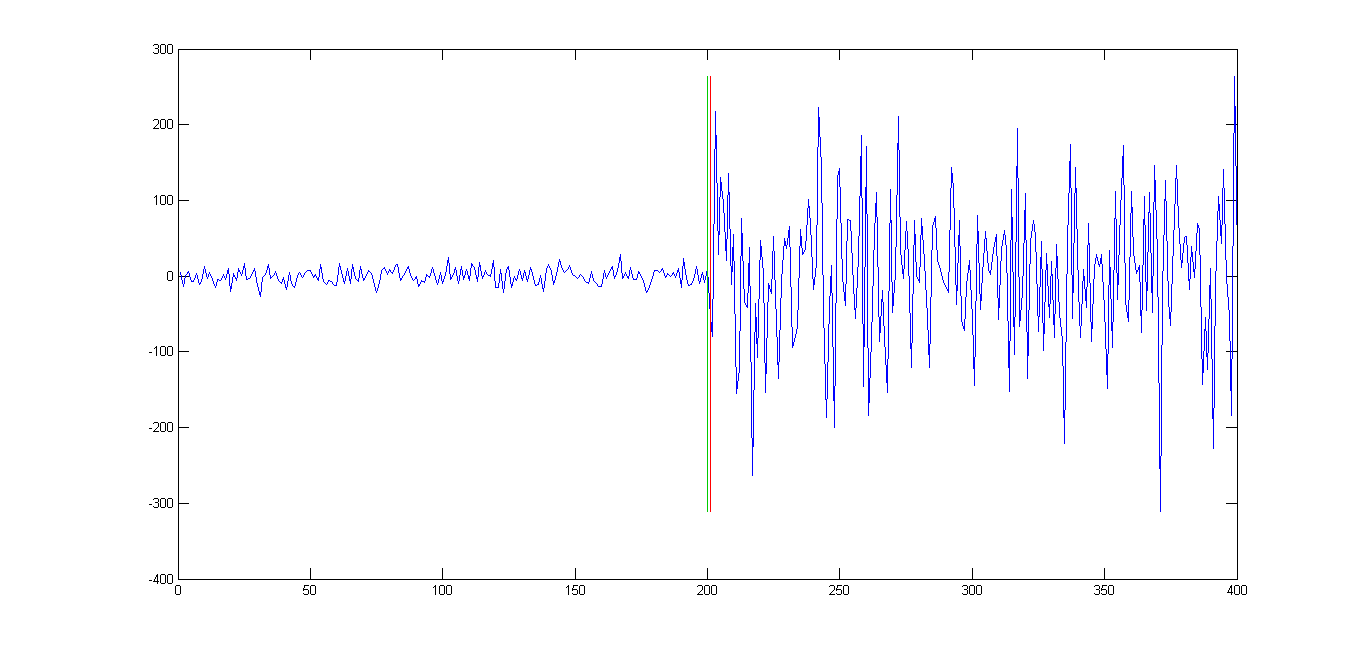
\includegraphics[scale=0.3]{cusum_1rupt.png}
		\caption{Détection d'une rupture par l'algorithme CUSUM}
	\end{figure}
\end{frame}

\section{Implémentations}

\subsection{Dichotomie}

\begin{frame}

\frametitle{Implémentation par dichotomie}

Principe : %détecter une rupture, séparer le signal en deux, détecter deux nouvelles ruptures, les comparer, etc., jusqu'à n ruptures.

\begin{itemize}
	\item[Maintenir] un ensemble de ruptures éligibles
	\item[Extraire] la meilleure rupture de cet ensemble
	\item[Calculer] les ruptures - éligibles - de chaque coté de la précédente
	\item[Boucler] jusqu'à avoir extrait suffisamment de ruptures
\end{itemize}

\begin{figure}
	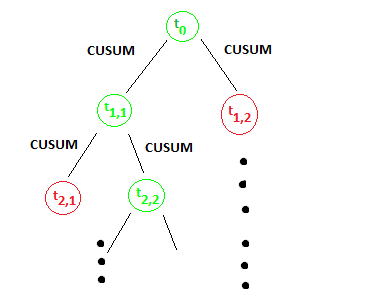
\includegraphics[scale=0.45]{diagramme_cusum_dikt.png}
	\caption{Principe du CUSUM dichotomique}
\end{figure}

%Avantages :
%\begin{itemize}
%	\item
%\end{itemize}

%Inconvénients :
%\begin{itemize}
%	\item
%\end{itemize}

\end{frame}

\begin{frame}
	\frametitle{Segmentation par dichotomie de signaux physiologiques}
	\begin{figure}
		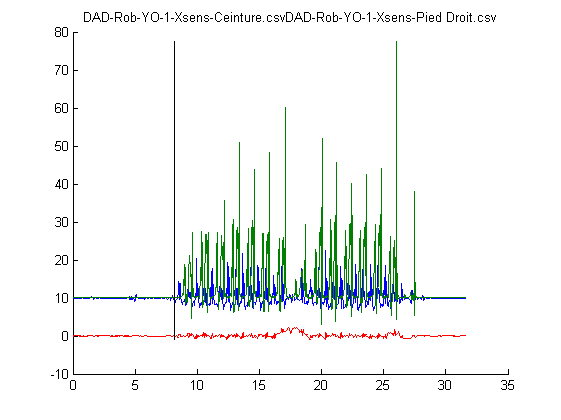
\includegraphics[scale=0.5]{dikt-seg1.png}
		\caption{Exemple d'une segmentation par CUSUM dichotomique
		~~~~
		(1 rupture)}
	\end{figure}
\end{frame}

\begin{frame}
	\frametitle{Segmentation par dichotomie de signaux physiologiques}
	\begin{figure}
		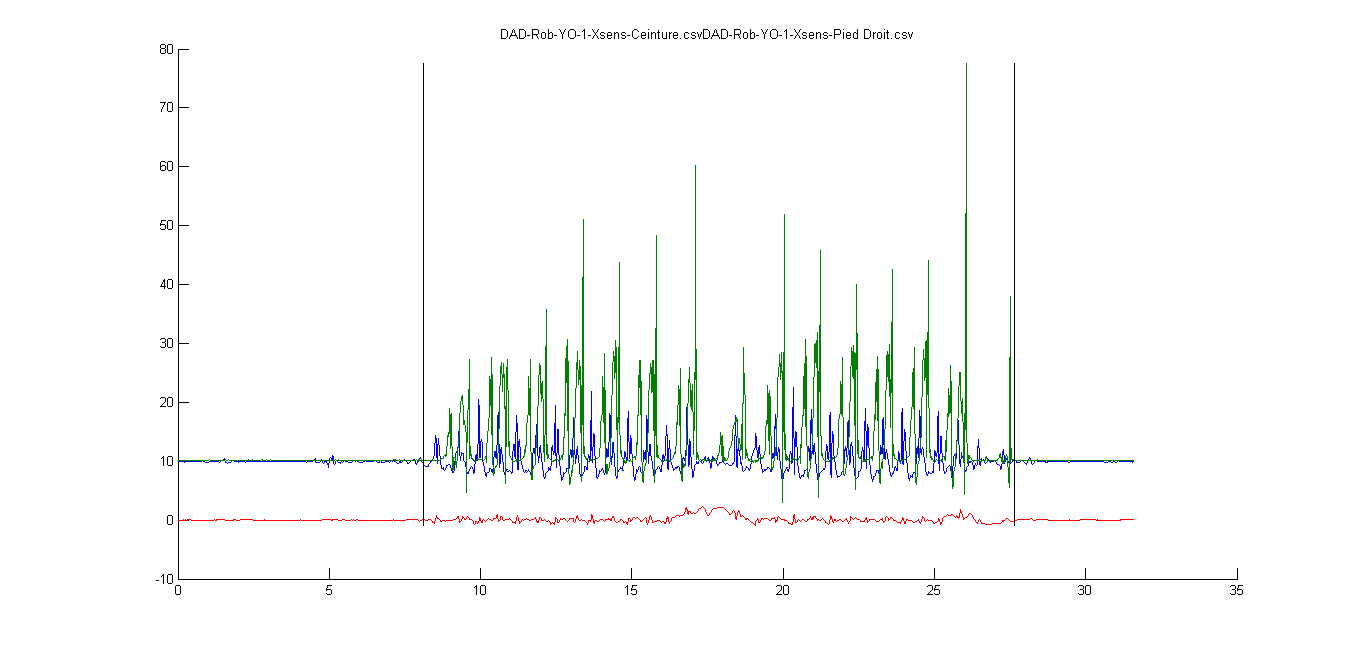
\includegraphics[scale=0.5]{dikt-seg2.png}
		\caption{Exemple d'une segmentation par CUSUM dichotomique 
		~~~~
		(2 ruptures)}
	\end{figure}
\end{frame}

\begin{frame}
	\frametitle{Segmentation par dichotomie de signaux physiologiques}
	\begin{figure}
		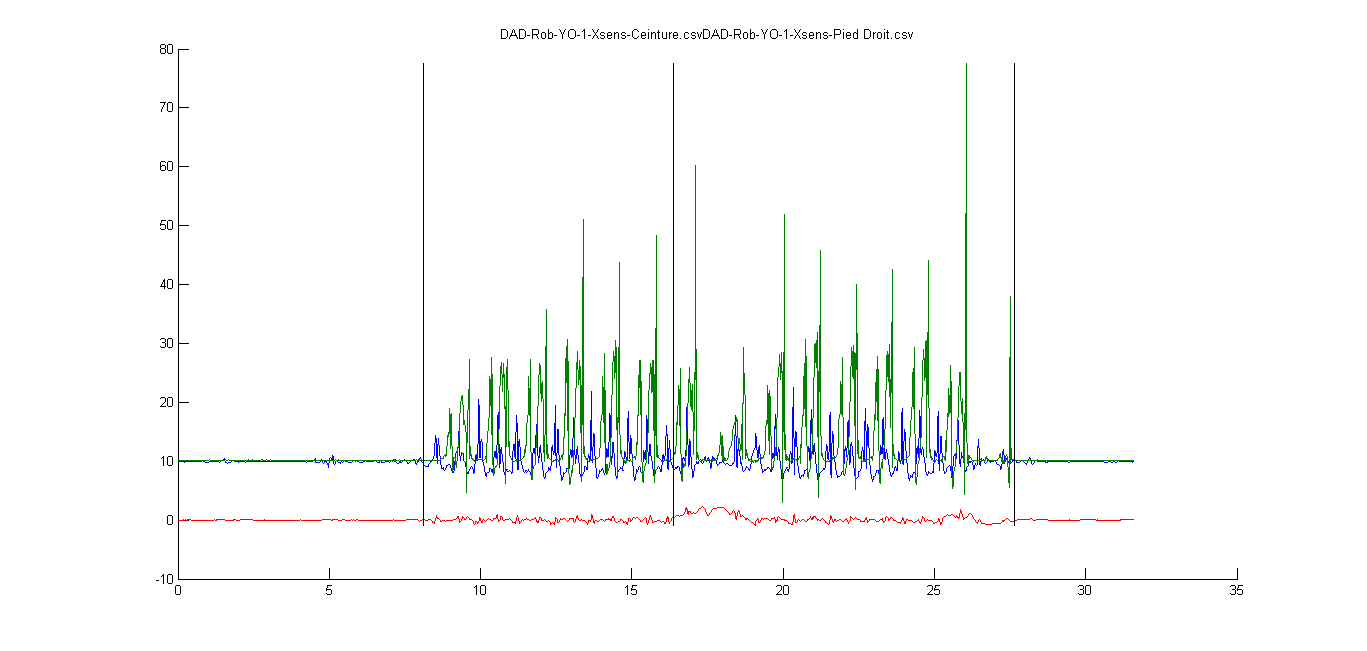
\includegraphics[scale=0.5]{dikt-seg3.png}
		\caption{Exemple d'une segmentation par CUSUM dichotomique
		~~~~
		(3 ruptures)}
	\end{figure}
\end{frame}

\begin{frame}
	\frametitle{Segmentation par dichotomie de signaux physiologiques}
	\begin{figure}
		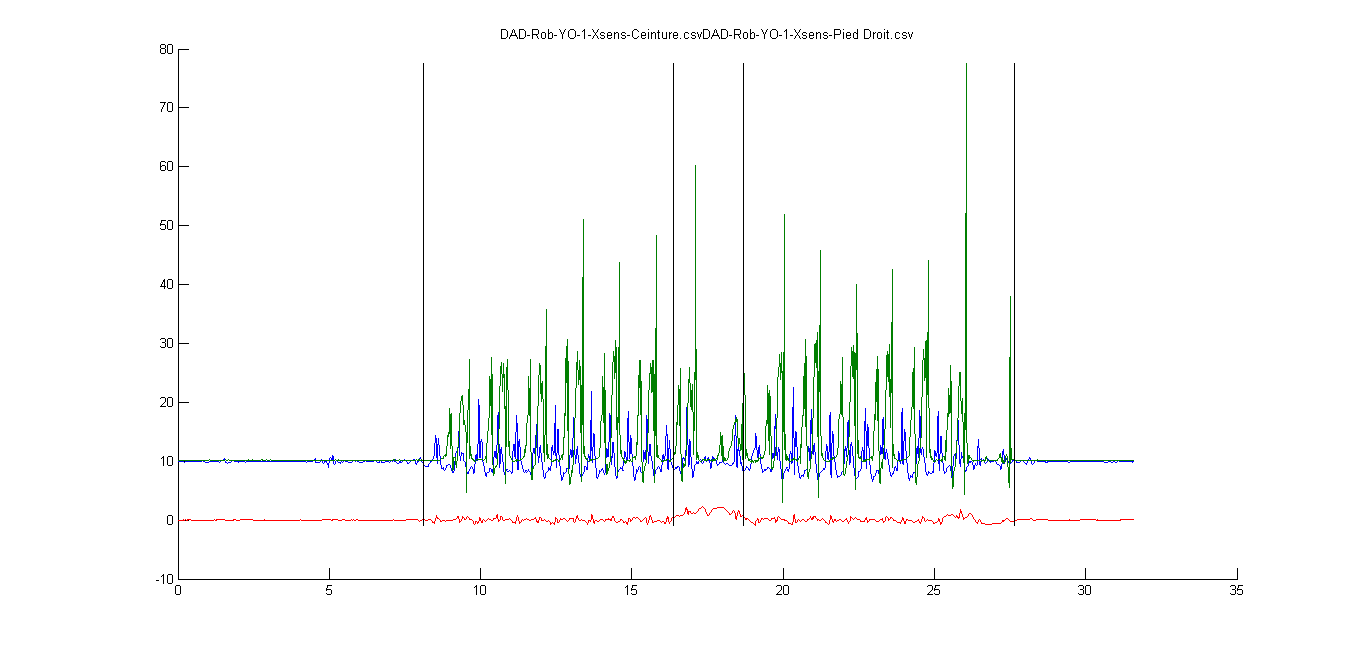
\includegraphics[scale=0.3]{dikt-seg4.png}
		\caption{Exemple d'une segmentation par CUSUM dichotomique
		~~~~
		(4 ruptures)}
	\end{figure}
\end{frame}

\begin{frame}
	\frametitle{Segmentation par dichotomie de signaux physiologiques}
	\begin{figure}
		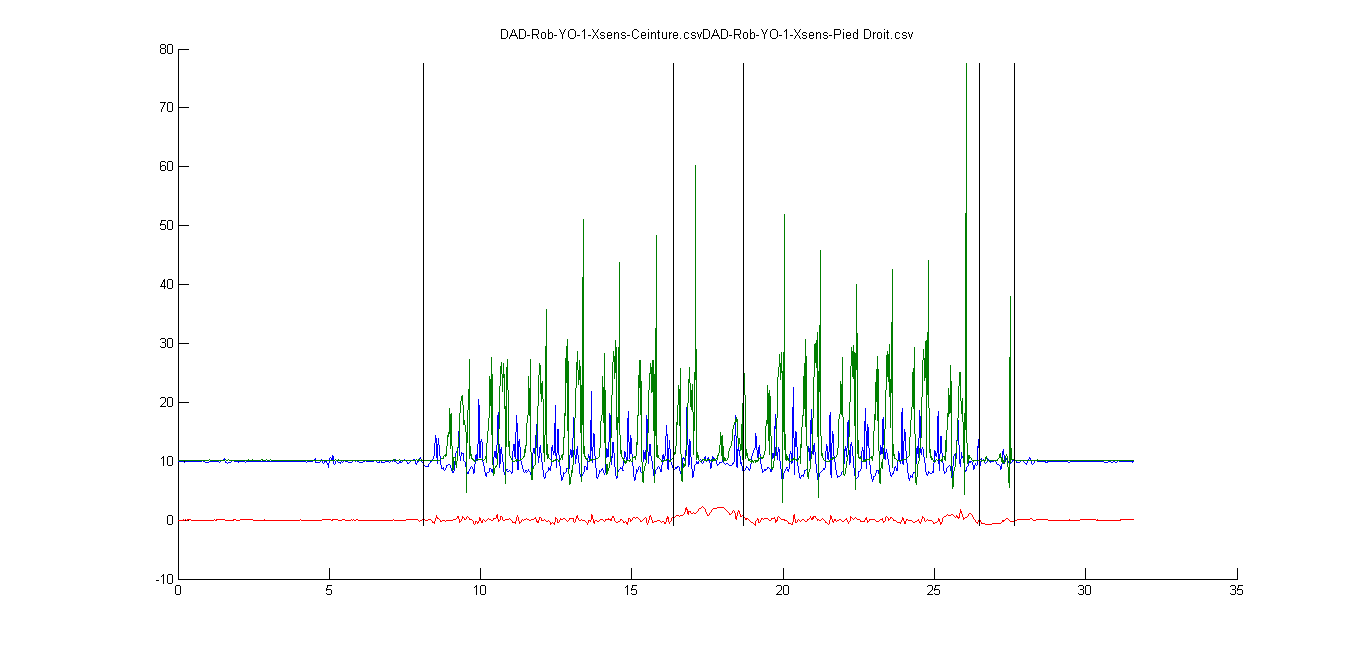
\includegraphics[scale=0.3]{dikt-seg5.png}
		\caption{Exemple d'une segmentation par CUSUM dichotomique
		~~~~
		(5 ruptures)}
	\end{figure}
\end{frame}

\begin{frame}
	\frametitle{Segmentation par dichotomie de signaux physiologiques}
	\begin{figure}
		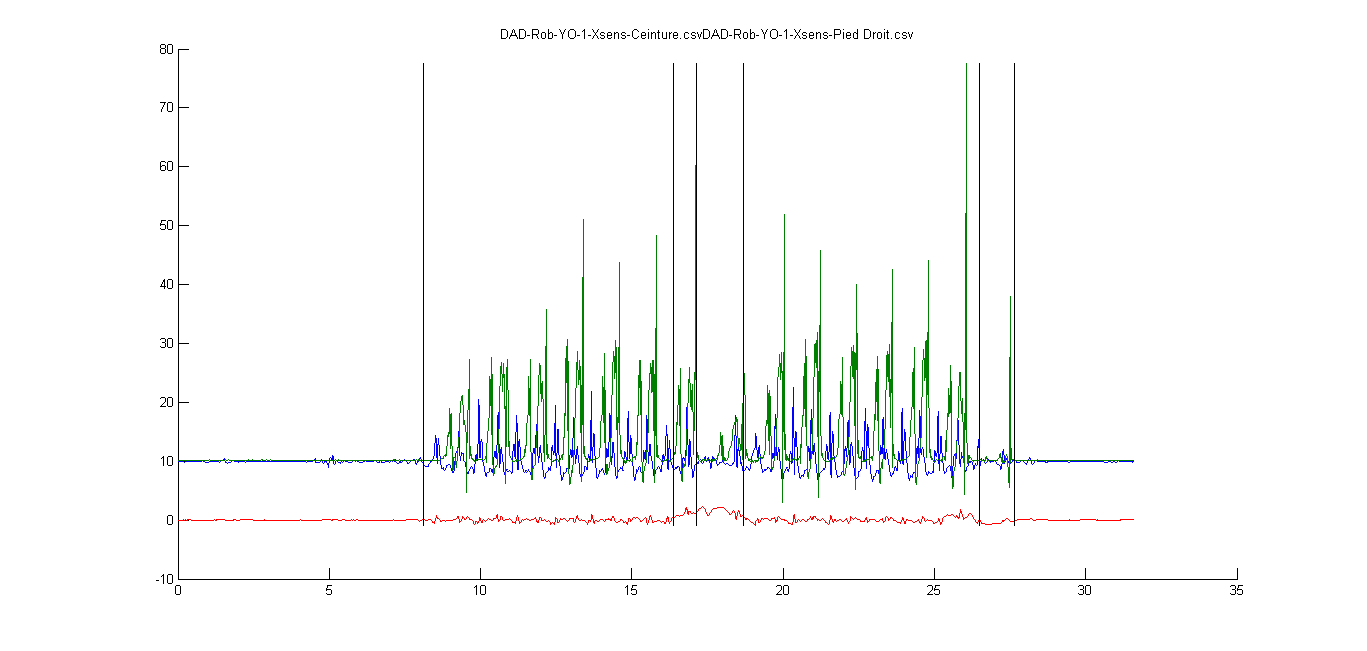
\includegraphics[scale=0.3]{dikt-seg6.png}
		\caption{Exemple d'une segmentation par CUSUM dichotomique
		~~~~
		(6 ruptures)}
	\end{figure}
\end{frame}

%\begin{frame}
%	\frametitle{Résultats : taux d'erreur}
%	\begin{figure}
%		\includegraphics{}
%		\caption{Taux d'erreurs entre vraie rupture et rupture détectée (CUSUM dichotomique)}
%	\end{figure}
%\end{frame}

\subsection{Fenêtres}

\begin{frame}

\frametitle{Implémentation par fenêtres}
Principe : %faire glisser une fenêtre de taille fixe le long du signal. Dans cette fenêtre, calculer le log-likelihood ratio associé au centre de la fenêtre. Rechercher ensuite les maximas.

\begin{itemize}
	\item[Fixer] une fenêtre de travail au début du signal
	\item[Calculer] le ratio d'une rupture au milieu de la fenêtre
	\item[Glisser] la fenêtre sur le signal en refaisant le calcul
\end{itemize}

\begin{figure}
	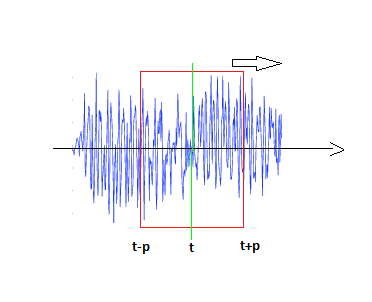
\includegraphics[scale=0.5]{diagramme_cusum_fen.png}
	\caption{Principe du CUSUM par fenêtres}
\end{figure}

%Avantages :
%\begin{itemize}
%	\item
%\end{itemize}

%Inconvénients :
%\begin{itemize}
%	\item
%\end{itemize}

\end{frame}

\begin{frame}
	\frametitle{Segmentation par fenêtre de signaux physiologiques}
	\begin{figure}
		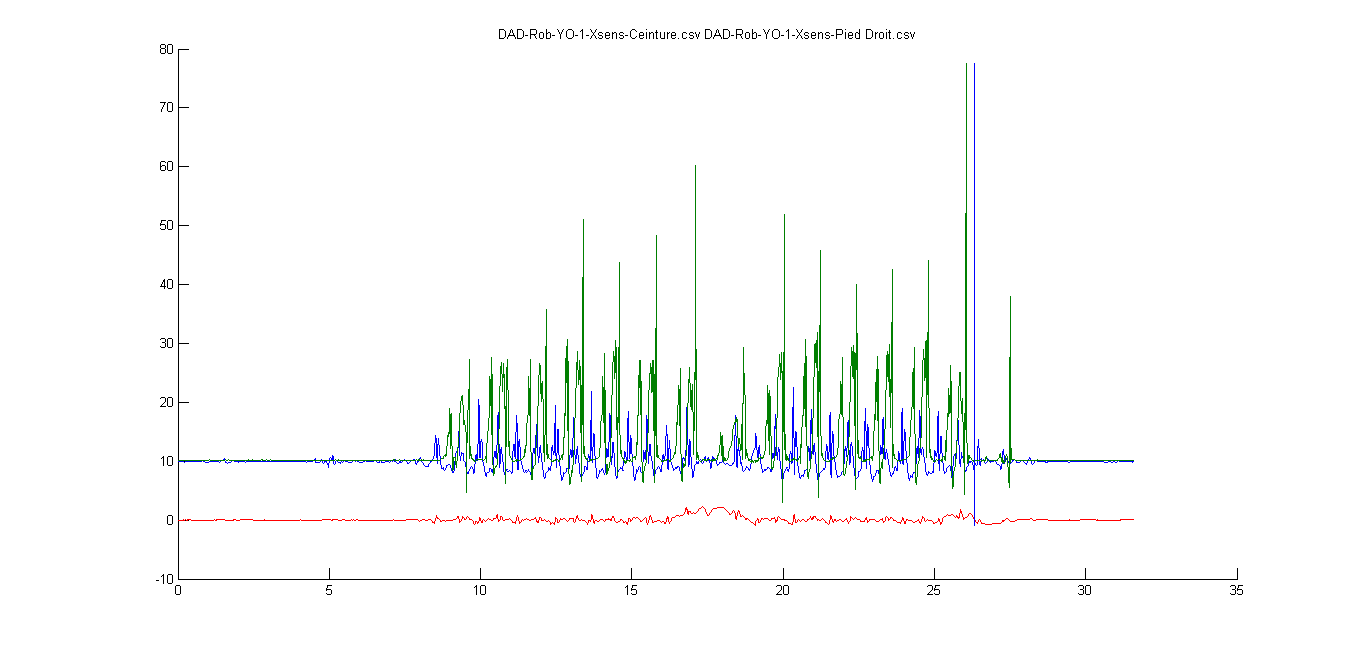
\includegraphics[scale=0.3]{seg1_win.png}
		\caption{Exemple d'une segmentation par CUSUM en fenêtres (1 rupture)}
	\end{figure}
\end{frame}

\begin{frame}
	\frametitle{Segmentation par fenêtre de signaux physiologiques}
	\begin{figure}
		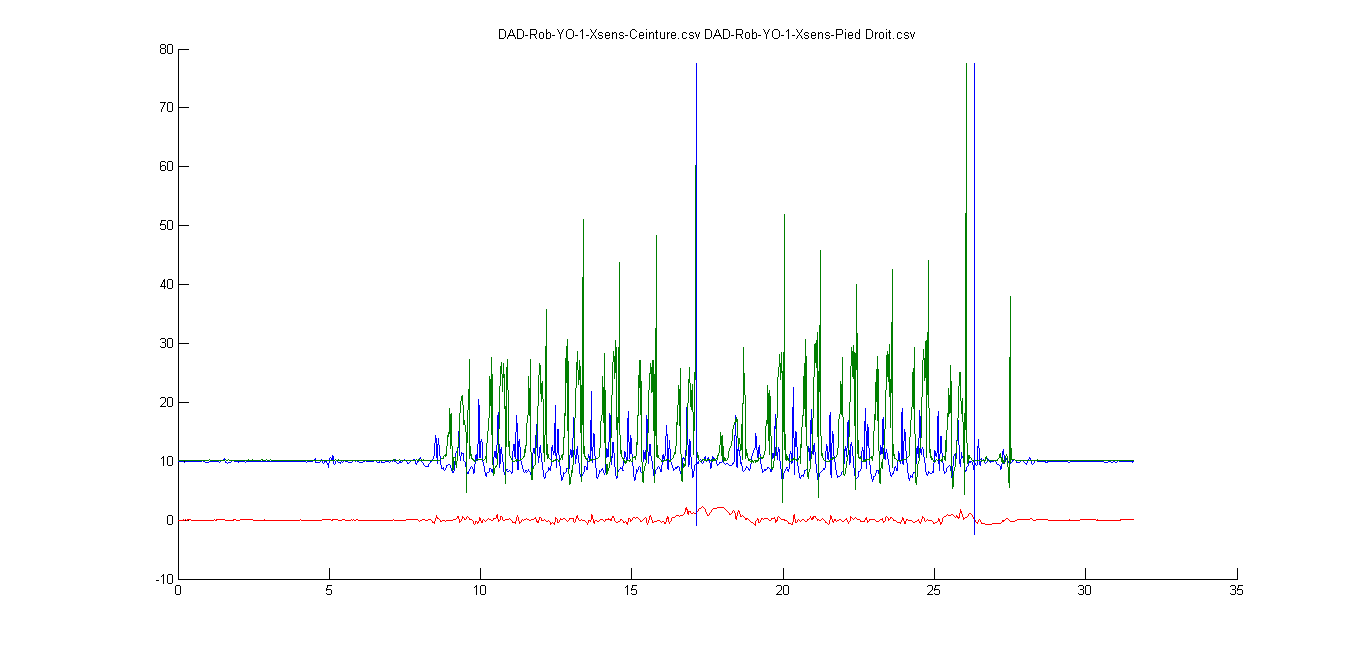
\includegraphics[scale=0.3]{seg2_win.png}
		\caption{Exemple d'une segmentation par CUSUM en fenêtres (2 ruptures)}
	\end{figure}
\end{frame}

\begin{frame}
	\frametitle{Segmentation par fenêtre de signaux physiologiques}
	\begin{figure}
		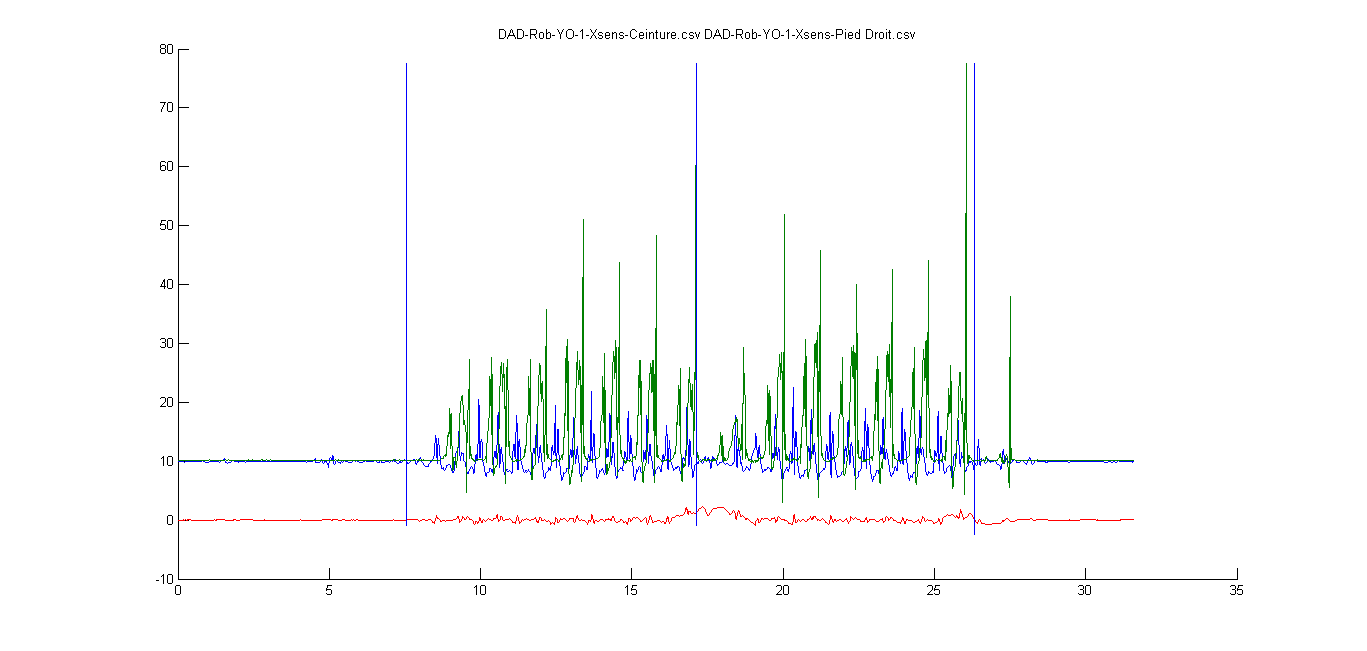
\includegraphics[scale=0.3]{seg3_win.png}
		\caption{Exemple d'une segmentation par CUSUM en fenêtres (3 ruptures)}
	\end{figure}
\end{frame}

\begin{frame}
	\frametitle{Segmentation par fenêtre de signaux physiologiques}
	\begin{figure}
		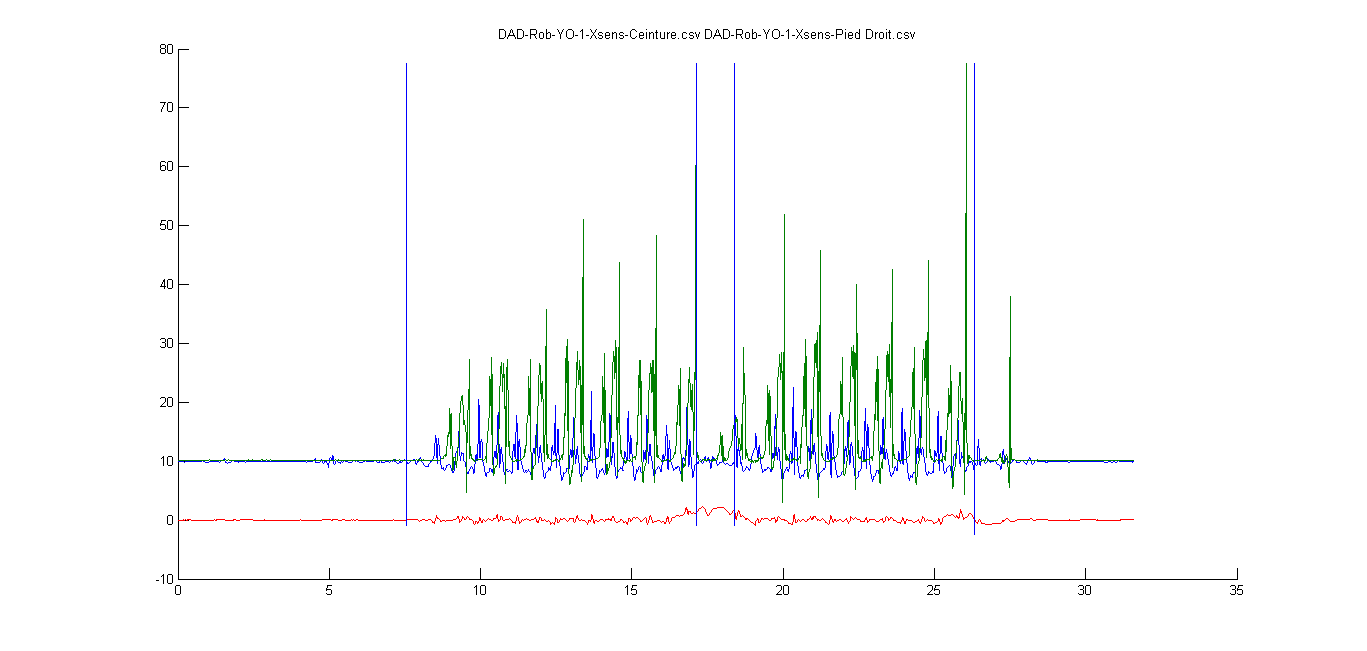
\includegraphics[scale=0.3]{seg4_win.png}
		\caption{Exemple d'une segmentation par CUSUM en fenêtres (4 ruptures)}
	\end{figure}
\end{frame}

\begin{frame}
	\frametitle{Segmentation par fenêtre de signaux physiologiques}
	\begin{figure}
		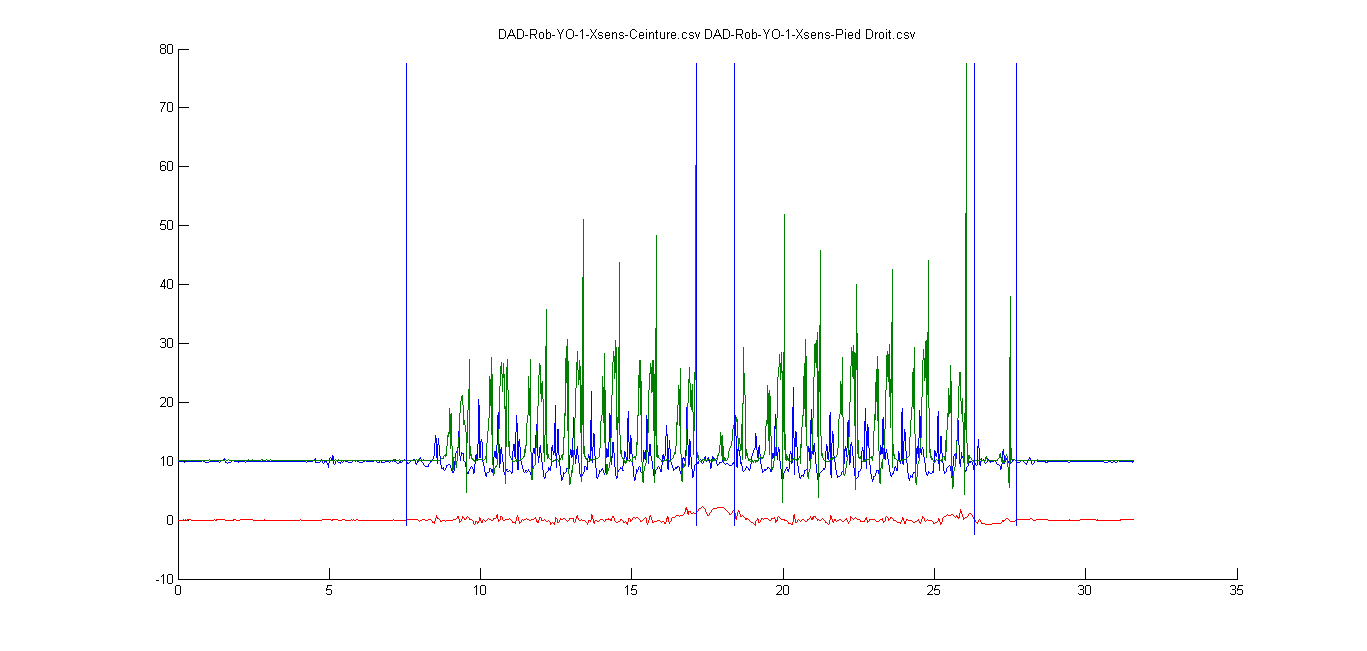
\includegraphics[scale=0.3]{seg5_win.png}
		\caption{Exemple d'une segmentation par CUSUM en fenêtres (5 ruptures)}
	\end{figure}
\end{frame}

\begin{frame}
	\frametitle{Segmentation par fenêtre de signaux physiologiques}
	\begin{figure}
		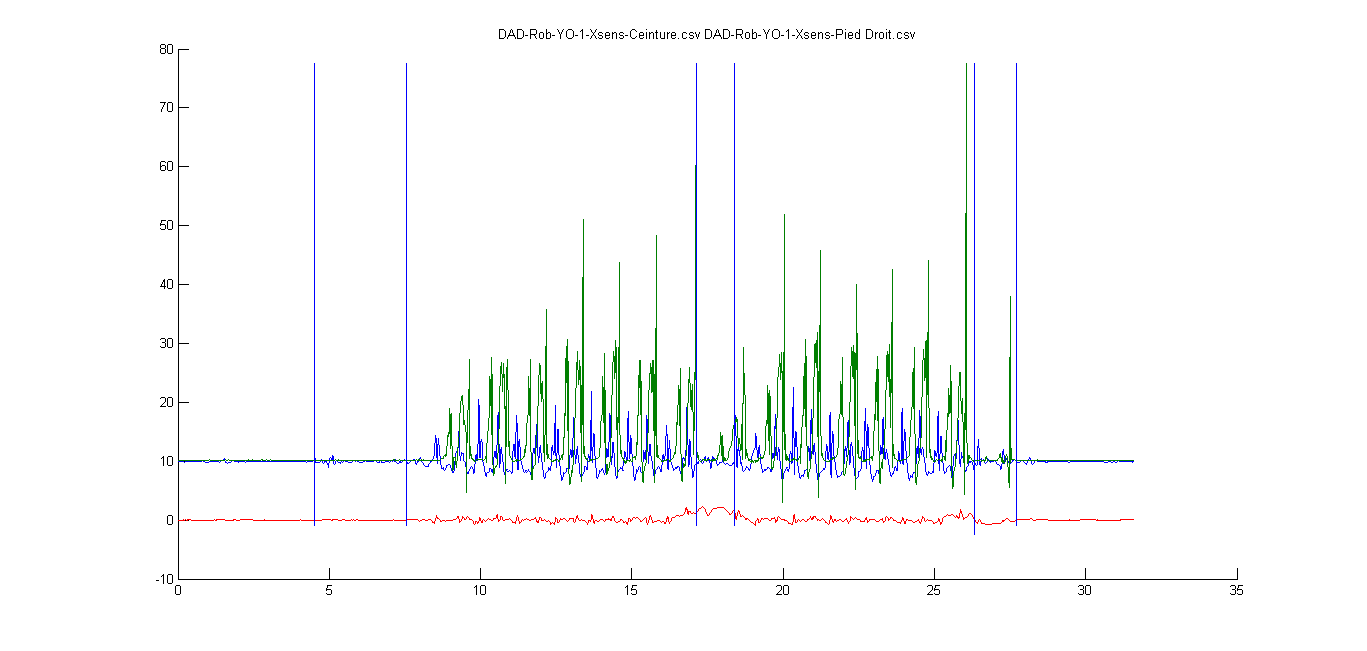
\includegraphics[scale=0.3]{seg6_win.png}
		\caption{Exemple d'une segmentation par CUSUM en fenêtres (6 ruptures)}
	\end{figure}
\end{frame}

%\begin{frame}
%	\frametitle{Résultats : taux d'erreur}
%	\begin{figure}
%		\includegraphics{}
%		\caption{Taux d'erreurs entre vraie rupture et rupture détectée}
%	\end{figure}
%\end{frame} 

\section{Conclusion}

\begin{frame}

\begin{itemize}

	\item[Approche] par dichotomie
			\\ Moins gourmande en calculs
			\\ Moins adaptée à la théorie de l'algorithme CUSUM
			\\ De nombreuses double-ruptures, des ruptures mal détectées
	
	\item[Approche] par fenêtres
			\\ Complexité plus élevée
			\\ Plus adaptée à la théorie
			\\ Plus performante pour des écarts entre deux ruptures légers
	
	\item[Capteurs] actuels à 100Hz : bonne détection
	
	\item[Travail] sur les segments : différencier et détecter les différents types de maladies
	\item[$\Longrightarrow$] machine learning sur les segments obtenus
	\vspace*{1cm}

\end{itemize}

\end{frame}

\end{document}